\subsection{Auswertung}
Für alle Messungen der $U$-$I$-Kennlinie wird $\sqrt{I-I_0}$ gegen die Gegenspannung $U_\mathrm{G}$ aufgetragen (Abbildung \ref{kennlinien1} und \ref{kennlinien2}). An die Daten wird eine Anpassungsgerade $\sqrt{I-I_0}=aU_\mathrm{G}+b$ angepasst.Für kleine Werte von $I-I_0$ wird der aus der Gauß'schen Fehlerfortpflanzung resultierende Fehler deutlich größer als die absoluten Fehlerschranken. Für diese Werte wurden die Fehlerschranken seperat berechnet. Die Anpassungsgeraden ändern sich dadurch nicht, da ohnehin nur Werte im linearen Bereich beachtet werden. Der Index an der Wellenlänge steht für den Messdurchlauf. Die aus der Anpassung folgenden Werte sind in Tabelle \ref{tab:photoeffekt} zu sehen. Aus den Parametern wird die Grenzspannung über $U_0=b/a$ berechnet. 

\newpage

\begin{table}[h]
  \centering
    \begin{tabular}{c c c c}
      \toprule
      $\lambda/\mathrm{nm}$ & $a\mathrm{V}/ \sqrt{\mathrm{nA}}$ & $b/\sqrt{\mathrm{nA}}$ & $U_0/V$\\
      \midrule
      $365_1$ & $2,08 \pm 0,03 $ &$3,47 \pm 0,01 $ & $1,67 \pm 0,02$\\
      $365_2$ & $2,22 \pm 0,03 $ &$3,52 \pm 0,03  $ & $1,59 \pm 0,02$\\
      $405_1$ & $1,71 \pm 0,01 $ &$2,39 \pm 0,01 $ & $1,39 \pm 0,01$\\
      $405_2$ & $1,86 \pm 0,01 $ &$2,398 \pm 0,009$ & $1,286 \pm 0,009$\\
      $436_1$ & $2,15 \pm 0,08 $ &$2,72 \pm 0,07  $ & $1,26 \pm 0,06  $\\
      $436_2$ & $2,622 \pm 0,009$ &$2,800 \pm 0,004$ & $1,068 \pm 0,004 $\\
      $546_1$ & $3,06 \pm 0,06 $ &$1,789 \pm 0,007$ & $0,58 \pm 0,01$\\
      $546_2$ & $2,4 \pm 0,1  $ &$1,34 \pm 0,03  $ & $0,54 \pm 0,03$\\
      $578_1$ & $2,08 \pm 0,07 $ &$0,992 \pm 0,008$ & $0,48 \pm 0,02$\\
      $578_2$ & $1,81 \pm 0,06 $ &$0,95 \pm 0,01$ & $0,53 \pm 0,02$\\
      \bottomrule
    \end{tabular}
    \caption{Parameter der Anpassungsgeraden}
    \label{tab:photoeffekt}
\end{table}

\begin{figure}[h!]
  \centering
  \begin{subfigure}[h]{0.5\textwidth}
    \centering
    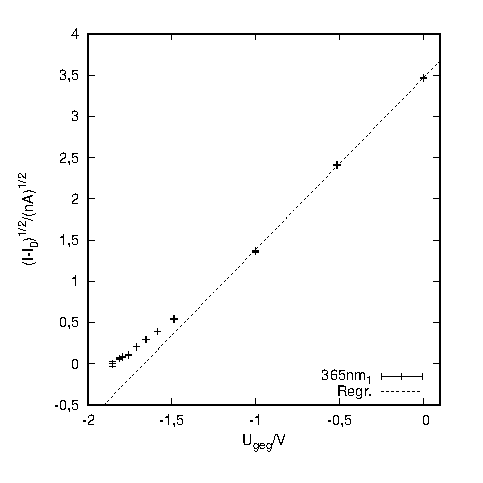
\includegraphics{data/Messung_photoeffekt/365nm_1.eps}
  \end{subfigure}%
  \begin{subfigure}[h]{0.5\textwidth}
    \centering
    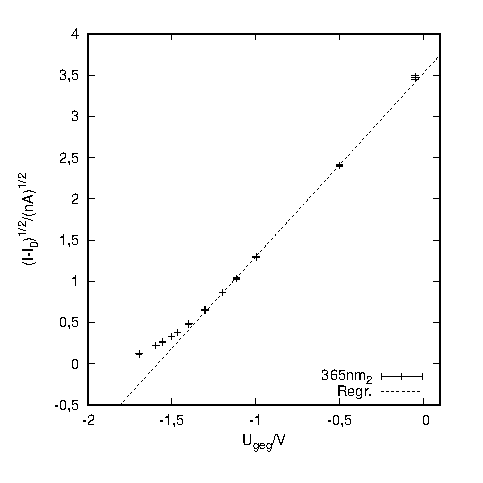
\includegraphics{data/Messung_photoeffekt/365nm_2.eps}
  \end{subfigure}
    \begin{subfigure}[h]{0.5\textwidth}
    \centering
    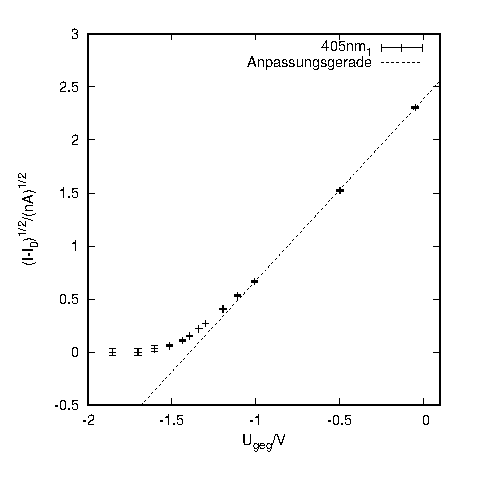
\includegraphics{data/Messung_photoeffekt/405nm_1.eps}
  \end{subfigure}%
  \begin{subfigure}[h]{0.5\textwidth}
    \centering
    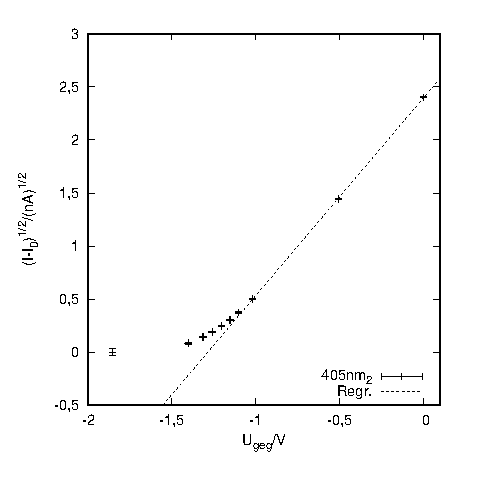
\includegraphics{data/Messung_photoeffekt/405nm_2.eps}
  \end{subfigure}
  \caption{Kennlinien für 365nm und 405nm}
  \label{kennlinien1}
\end{figure}

\newpage
\vfill

\begin{figure}[hbt]
   \begin{subfigure}[h]{0.5\textwidth}
    \centering
    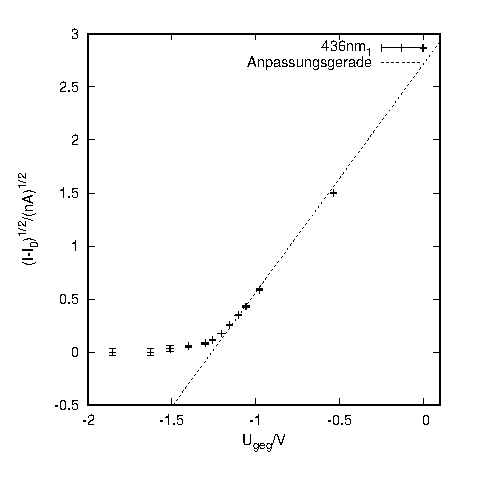
\includegraphics{data/Messung_photoeffekt/436nm_1.eps}
  \end{subfigure}%
  \begin{subfigure}[h]{0.5\textwidth}
    \centering
    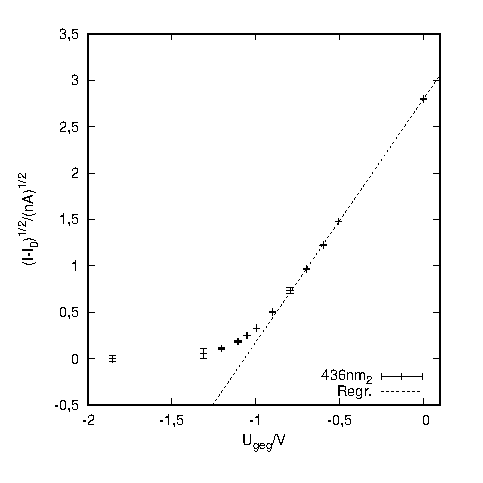
\includegraphics{data/Messung_photoeffekt/436nm_2.eps}
  \end{subfigure}
  \begin{subfigure}[h]{0.5\textwidth}
    \centering
    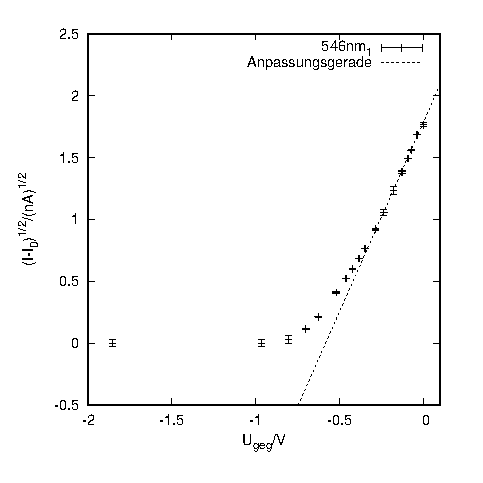
\includegraphics{data/Messung_photoeffekt/546nm_1.eps}
  \end{subfigure}%
  \begin{subfigure}[h]{0.5\textwidth}
    \centering
    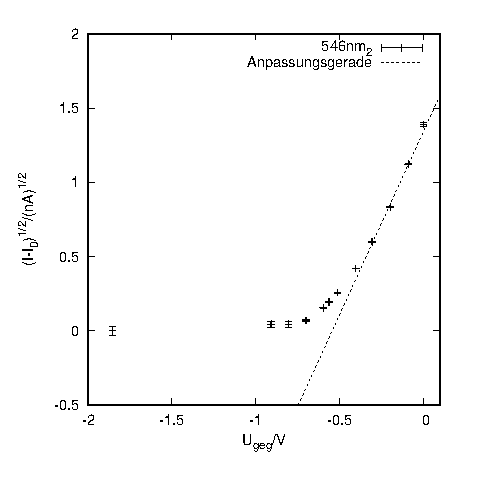
\includegraphics{data/Messung_photoeffekt/546nm_2.eps}
  \end{subfigure}
  \begin{subfigure}[h]{0.5\textwidth}
    \centering
    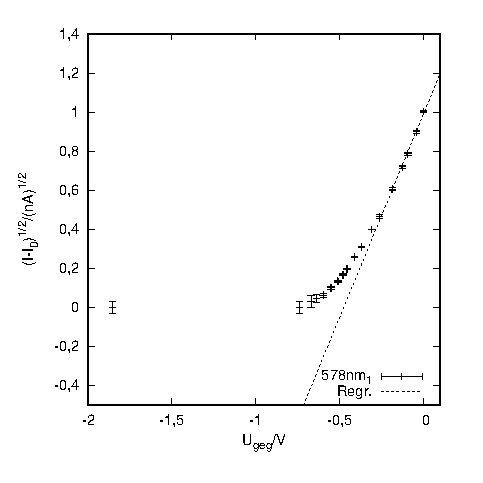
\includegraphics{data/Messung_photoeffekt/578nm_1.eps}
  \end{subfigure}%
  \begin{subfigure}[h]{0.5\textwidth}
    \centering
    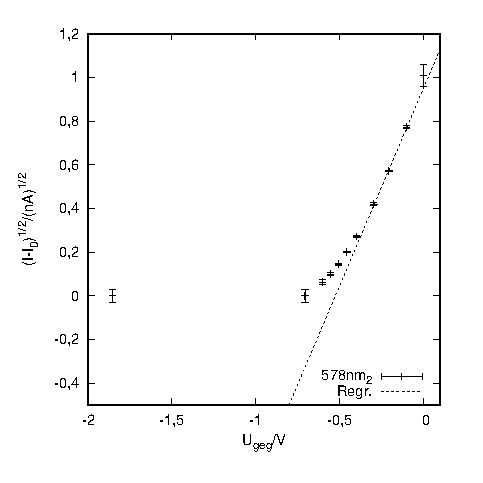
\includegraphics{data/Messung_photoeffekt/578nm_2.eps}
  \end{subfigure}%
  \caption{Kennlinien für 436nm, 546nm und 578nm}
  \label{kennlinien2}
\end{figure}

\vfill
\clearpage

Für jede Wellenlänge wird der varianzgewichtete Mittelwert der Grenzspannung $U_0$ berechnet. Dann wird die Grenzspannung gegen die Frequenz $\nu$ aufgetragen und eine Gerade $U_0=a\nu+b$ angepasst (siehe Abbildung \ref{planck}). Die Parameter sind: 
\begin{align*}
  a&=(3,8 \pm 0,2)10^{-15}\mathrm{Vs}\\  
  b&=(-1,5 \pm 0,2) \mathrm{V}
\end{align*}

\begin{figure}[h]
  \centering
  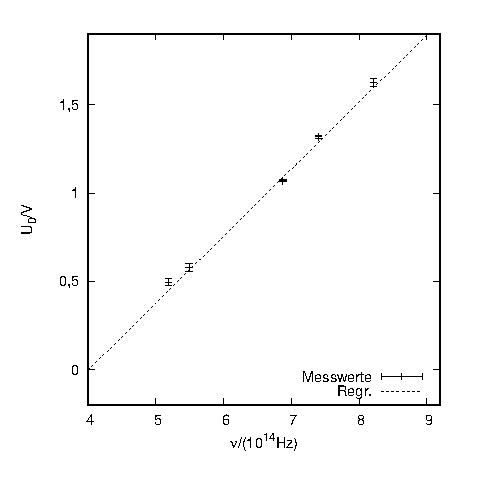
\includegraphics[width=8cm]{data/Messung_photoeffekt/f_u.eps}
  \caption{Grenzspannung und Austrittsarbeit beim Photoeffekt}
  \label{planck}
\end{figure}


Mit Gleichung \ref{eqn:grenzspannung} lassen sich nun das Plancksche Wirkungsquantum und die Austrittsarbeit berechnen:
\begin{align*}
  h&=ea=(6,08 \pm 0,03)10^{-34}\mathrm{Js}\\
  W_\mathrm{A}&=-eb=(1,5 \pm 0,2)\mathrm{eV}
\end{align*}

Der Literaturwert für das Wirkungsquantum ist $h=6,63 \cdot 10^{-34}\mathrm{Js}$. Unser Wert weicht also um ca. $8\%$ ab. Der tatsächliche Wert liegt allerdings nicht im Fehlerbereich. Dies liegt vermutlich daran, dass händisch der lineare Bereich für die Ermittlung der Grenzspannung ausgewählt werden musste. Bereits das Hinzunehmen oder Entfernen weniger Messpunkte hat deutliche Auswirkungen auf die Grenzspannung. Dieser Fehler hätte durch eine höhere Zahl der Messpunkte im linearen Bereich verringert werden können. \\ \\
Vermutlich handelt es sich bei dem Versuch um den Aufbau aus \cite{leybold}. Das Anodenmaterial wäre also Platin mit einer Austrittsarbeit von ca. $5,66$eV \cite{kalium}. Dieser Wert liegt außerhalb unserer Fehlergrenzen, vermutlich aus dem gleichen Grund wie für das Wirkungsquantum. \\ \\

Die $U$-$I$-Kennlinie bei $365$nm und verringerter Intensität ist in Abbildung \ref{fig:lowintensity} zu sehen. Die Parameter der Anpassungsgerade und die Grenzspannung sind:
\begin{align*}
  a&=(1,32 \pm 0,01)\sqrt{\mathrm{nA}}/\mathrm{V}\\
  b&=(2,07 \pm 0,01)\sqrt{\mathrm{nA}}\\
  U_0&=(1,57 \pm 0,02)\mathrm{V}   
\end{align*}

Es ist zu sehen, dass sich die Grenzspannung trotz der Intensitätsänderung kaum verändert hat, die Kennlinie entspricht also einfach einem Vielfachen der Ursprünglichen Kennlinie. Dieses Verhalten wurde auch erwartet, da sich durch die Erhöhung der Intensität die Zahl der Photonen und somit die Zahl der herausgelösten Elektronen erhöht, die Energie der einzelnen Elektronen aber gleich bleibt.

\begin{figure}[h]
  \centering
  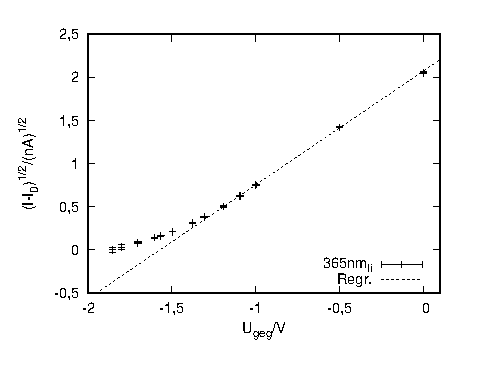
\includegraphics[width=8cm]{data/Messung_photoeffekt/365nm_low_intensity.eps}
  \caption{Kennlinie für 365nm und verringerte Intensität}
  \label{fig:lowintensity}
\end{figure}
